\subsection{\Home page}
	Dette afsnit vil indeholde en gennem gang af design, grafisk bruger interface og implentering af Home page activity til android applikationen
	\subsubsection{Design}
	HomeActivity er bygget op om samme design som LogIn, der er dog tilføjet et fragment for hver af de to tabs i layoutet. Fragmentet opfører sig som en selvstændig activity, som lever i HomeActivity. \\
	HomeActivity bruger interfacet IUserPreference til at hente bruger oplysninger ned, og gemme dem.\\
	Strukturen af HomeActivity kan ses på figur \ref{fig:Klasse diagram for HomeActivity}
	\begin{figure}[h!]
		\begin{center}
			\includegraphics[height=8cm]{Android/Billeder/clHomeActivity}
		\end{center}
		\caption{Fragment struktur for HomeActivity}
		\label{fig:Klasse diagram for HomeActivity}
	\end{figure}
	\pagebreak
	
	\subsubsection{Grafisk Bruger Interface}
	Hjemsiden er noget mere kompleks end nogle af de andre siger. Dette er forsøgt at gjort simpelt ved ikke at have for mange egenskaber af gangen.
	\begin{figure}[h!]
		\begin{center}
			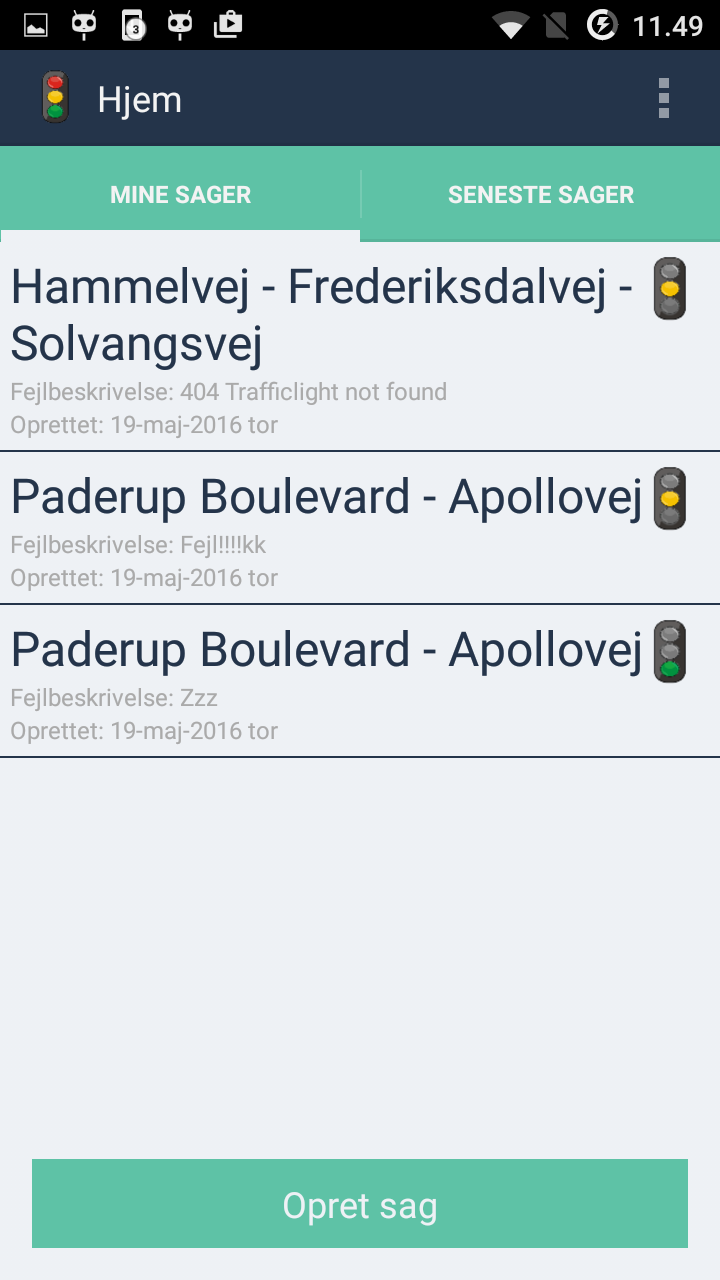
\includegraphics[height=8cm]{Android/Billeder/AndroidHomePage}
		\end{center}
		\caption{Traffic Control - Home Page}
		\label{fig: Traffic Control - Home Page}
	\end{figure}
	\\
	Hjemsiden indeholder en liste af sager. Trafik lyset ud for sagen viser hvilken status den er i. Rød for lukket, gul for afventer og grøn for åben. \\
	Der er to taps hvor man kan vælge at se alle sager eller om man kun vil se de sager man selv har taget.
	\\Der kan findes en menu, hvis man trækker fra venstre mod højre, hvor navigation til resten af app'en kan foretages.
	
	
	\subsubsection{Implementering} \label{HomePageImp}
	HomeActivity er også bygget op omkring MVP, hvor sager bliver gemt i modellen. Modellen indeholder de sager der er tilknyttet brugeren som er logget ind, samt de seneste 1000 sager. Alt data hentes fra DAL-laget.
	\\For at kunne vise "Mine sager" og "Alle sager" på en fornuftig måde, består HomeActivity af to fragmenter. Som hver især har en presenter og en model, altså samme design som LogInActivity på figur \vref{fig:Klasse diagram for Log Ind Android}.
	\\Der er lavet en Drawer menu i venstre side, til navigation af app'en. Funktionallitet og layout til menuen er lavet i klassen MenuActivity, som HomeActivity nedarver fra, og derved har HomeActivity menu funktionallitet.
	Et klassediagram for dette, kan ses på figur \vref{fig:Klasse diagram for HomeActivity}.
	 
	\pagebreak